%*************************************************
% A template for PhD and MSc thesis. V1.0.
% Please see "guideline.pdf" first.
%*************************************************
% Iman Izadi, 1394
% Dept. of Electrical and Computer Engineering, IUT
%*************************************************
% این قالب بر اساس "شیوه‌نامه تدوین پایان‌نامه‌ها و رساله‌های 
%تحصیلات تکمیلی" دانشگاه صنعتی اصفهان تهیه شده است
%*************************************************

\documentclass[a4paper,fleqn]{report} 
%\usepackage{refcheck}

% All the packages and general definitions are included in this file: preamble.tex
%*************************************************
% All the packages and definitions are included here.
%*************************************************
%*************************************************
% Iman Izadi, 1394
% Dept. of Electrical and Computer Engineering, IUT
%*************************************************

\usepackage{amsthm,amssymb,amsmath}			% Writing math
\usepackage{epsf,graphicx}									% Including graphics
\usepackage[a4paper]{geometry}							% Fixing page layout and margins
\usepackage{titlesec}											% Change chapter and section titles
\usepackage{setspace}											% Change line spacing
\usepackage[stable,bottom]{footmisc}					% Move footnotes to the bottom of page

\usepackage{zref-perpage}									% Reset footnote counter in each page
\zmakeperpage[1]{footnote}

\usepackage{xepersian}										% Persian
\settextfont{XB Zar}												% Persian font


% Use English digits in equations
\DefaultMathsDigits

% Default footnotes from left to right
\setfootnoteLR

% Use English numbers for English footnotes
\makeatletter
\def\@makeLTRfnmark{\hbox{\@textsuperscript{\latinfont\@thefnmark}}}
\renewcommand\@makefntext[1]{%
    \parindent 1em%
    \noindent
    \hb@xt@1.8em{\hss\if@RTL\@makefnmark\else\@makeLTRfnmark\fi}#1}
\makeatother

% Use dash instead of dot in section numbers
\SepMark{-}										

% Change fonts and margins of section and subsection titles
% For chapters please see firstpages.tex
\titlespacing*{\section}{0pt}{1cm}{0.2cm}
\titleformat{\section}
  {\fontsize{12}{6}\scshape\bfseries}{\thesection}{1em}{}

\titlespacing*{\subsection}{0pt}{.8cm}{0cm}
\titleformat{\subsection}
  {\fontsize{11}{6}\scshape\bfseries}{\thesubsection}{1em}{}
  
% Fix table of contents for chapters
\makeatletter 
\def\@chapter[#1]#2{\ifnum \c@secnumdepth >\m@ne
     \refstepcounter{chapter}%
     \typeout{\@chapapp\space\thechapter.}%
     \addcontentsline{toc}{chapter}%
       	{\@chapapp~\protect\numberline{\tartibi{chapter}\,:\space #1}}
  \else
  	 \addcontentsline{toc}{chapter}{#1}%
  \fi
  \chaptermark{#1}%
  \addtocontents{lof}{\protect\addvspace{10\p@}}%
  \addtocontents{lot}{\protect\addvspace{10\p@}}%
  \@makechapterhead{#2}%
  \@afterheading}
\makeatother
							

\begin{document}

% The first pages (before abstract) are included in this file: firstpages.tex
%*************************************************
% In this file the first few pages are typeset.
% Make the changes accordingly
%*************************************************

% شماره صفحات با حروف
\pagenumbering{adadi}

%***************************
% 1st page: Blank
%***************************
\thispagestyle{empty}
\mbox{}
\pagebreak

%***************************
% 2nd page: Besmelah
%***************************
\thispagestyle{empty}
\begin{center}
	~\vfill
	
\includegraphics[scale=1]{besm1.jpg}
	~\vfill
\end{center}
\pagebreak

%***************************
% 3rd page: Title
%***************************
\thispagestyle{empty}
%\pagenumbering{gobble}
\newgeometry{left=3cm,right=3cm,top=2cm}
\begin{center}

\includegraphics[height=3cm]{iut_logo.png}
\vspace{0.4cm}

\textbf{دانشگاه صنعتی اصفهان}\\
\vspace{0.4cm}

{\large

	دانشکده مهندسی برق و کامپیوتر
}
\vspace{3.5cm}

{\Large
	\textbf{بررسی راه‌های افزایش بهره‌وری در سیستم‌های با بهره‌وری پایین}\\
}
\vspace{3.5cm}

{\Large
	پایان‌نامه کارشناسی ارشد مهندسی برق -- کنترل\\
}
\vspace{1cm}

{\large
	\textbf{آذین آزاده}\\
}
\vspace{3.5cm}

{\large
	استاد راهنما\\
}
\vspace{0.5cm}

{\large
	\textbf{دکتر بهرام برزو}\\
}
\vspace{4cm}

\textbf{1394}

\end{center}
\restoregeometry
\pagebreak

%***************************
% 4th page: Signatures
%***************************
\thispagestyle{empty}
\newgeometry{left=3cm,right=3cm,top=2cm}
\begin{center}

\includegraphics[height=3cm]{iut_logo.png}
\vspace{0.4cm}

\textbf{دانشگاه صنعتی اصفهان}\\
\vspace{0.4cm}

{\large
	دانشکده مهندسی برق و کامپیوتر
}
\vspace{1.8cm}

\vfill

{\Large
	پایان‌نامه کارشناسی ارشد رشته مهندسی برق -- کنترل خانم آذین آزاده\\
	\vspace{.3cm}
	تحت عنوان\\
}


\end{center}
\vfill
\vspace{2.5cm}

{\large
	\textbf{بررسی راه‌های افزایش بهره‌وری در سیستم‌های با بهره‌وری پایین}
}

\vspace*{2cm}

در تاریخ 1394/1/1 توسط کمیته تخصصی زیر مورد بررسی و تصویب نهایی قرار گرفت:\\
\vspace{0.8cm}

{\normalsize
	
	\begin{tabular}{rr}
	\vspace*{.8cm}
	1- استاد راهنمای پایان‌نامه  & \hspace{2cm} دکتر بهرام برزو \\
	\vspace{.8cm}
	2- استاد مشاور پایان‌نامه  &\hspace{2cm} دکتر پوریا پرنیانی \\
	\vspace{.8cm}
	3-استاد داور (اختیاری) &\hspace{2cm} دکتر تهمتن ترابی \\
	\vspace{.8cm}
	۴-استاد داور (اختیاری) &\hspace{2cm} دکتر ثریا ثنایی\\
	\vspace{.8cm}
	سرپرست تحصیلات تکمیلی دانشکده &\hspace{2cm} دکتر جمشید جهانگیر\\
	\end{tabular}
}
\restoregeometry
\pagebreak

%***************************
% 5th page: Acknowledgment
%***************************
\thispagestyle{empty}
\newgeometry{left=3cm,right=4cm,top=4cm}
\vspace*{1.5cm}

{\large
	\textbf{تشکر و قدردانی}\\

	
پروردگار منّان را سپاسگزارم ......

}
\restoregeometry
\pagebreak

%***************************
% 6th page: Rights
%***************************
\thispagestyle{empty}
\newgeometry{left=6cm,right=6cm}

\begin{spacing}{3}
\leavevmode
\vfill
\parbox{8 cm}{

\textbf{\Large کلیه حقوق مادی مترتب بر نتایج مطالعات، ابتکارات و نوآوری‌های ناشی از تحقیق موضوع این پایان‌نامه  متعلق به دانشگاه صنعتی اصفهان است.}

}
\vfill
\end{spacing}
\restoregeometry
\pagebreak

%***************************
% 7th page: Dedication
%***************************
\thispagestyle{empty}
\vspace*{4cm}

{\LARGE
\centering
\textbf{تقدیم به \\ پدر و مادر عزیزم }

}
\pagebreak

%***************************
% 8th page: Table of contents
%***************************

\titleformat{\chapter}[display]
	{\normalfont\LARGE\bfseries\centering}{\chaptertitlename ~ \tartibi{chapter}}{20pt}{\LARGE}
\newgeometry{left=2.5cm,right=3cm,top=3cm,bottom=2.5cm,includehead=false,headsep=1cm,footnotesep=.5cm}
\baselineskip=.7cm

\addtocontents{toc}{\textbf{\underline{عنوان}}}
\addtocontents{toc}{\hfill\textbf{\underline{صفحه}}\par}
\addcontentsline{toc}{section}{فهرست مطالب}
\tableofcontents
\pagebreak

\addcontentsline{toc}{section}{فهرست تصاویر}
\listoffigures
\pagebreak

%\addcontentsline{toc}{section}{فهرست جداول}
%\listoftables
%\pagebreak

% change the font and margins of a chapter title
\titlespacing*{\chapter}{0pt}{3.5cm}{6cm}
\titleformat{\chapter}[display]
	{\normalfont\LARGE\bfseries\raggedright}{\chaptertitlename ~ \tartibi{chapter}}{20pt}{\LARGE}

% No page numbers on the first page of a chapter
\assignpagestyle{\chapter}{empty}
							

% The abstract of the paper goes here: abstract.tex
%*************************************************
% In this file the abstract is typeset.
% Make changes accordingly.
%*************************************************

\addcontentsline{toc}{section}{چکیده}
\newgeometry{left=2.5cm,right=3cm,top=3cm,bottom=2.5cm,includehead=false,headsep=1cm,footnotesep=.5cm}
\setcounter{page}{1}
\pagenumbering{arabic}						% شماره صفحات با عدد
\thispagestyle{empty}

~\vfill

\subsection*{چکیده}
\begin{small}
\baselineskip=0.7cm

در سال‌های اخیر استفاده از انرژی‌های تجدید‌پذیر و جایگزین کردن آن‌ها به جای سوخت‌های فسیلی در کشور‌های توسعه‌یافته و صنعتی با رشد قابل توجهی همراه بوده است. یکی از این انرژی‌های تجدید‌پذیر که بیشتر از سایر انرژی‌ها مورد استفاده قرار گرفته، انرژی باد است. توربین‌های بادی سیستم‌های الکترومکانیکی پیچیده‌ای هستند که انرژی باد را به انرژی الکتریکی تبدیل می‌کنند و از این رو بخش‌های مختلف توربین‌های بادی در معرض عیب‌های مختلفی  قرار می‌گیرند. از آنجایی‌ که زیر‌سیستم‌های مختلف توربین بادی با یکدیگر در ارتباط هستند، با ظهور عیب در یک زیر‌سیستم توربین بادی، امکان پخش شدن و اثر‌گذاری آن عیب در کل سیستم وجود دارد. از این رو برای جلوگیری و کاهش هزینه‌های ناشی از وقوع عیب در سیستم، نیازمند مکانیزمی هستیم که عیب را در لحظات ابتدایی وقوع در سیستم شناسایی کرده و به رفع اثر آن بپردازد. روش‌های تشخیص و جداسازی عیب در سیستم‌ها به دو دسته‌ی کلی مبتنی بر مدل و مبتنی بر سیگنال تقسیم می‌شوند. یکی از روش‌های مبتنی بر مدل برای شناسایی عیوب یک سیستم، استفاده از رویتگر‌های ورودی ناشناخته است. در این روش به کمک مدل سیستم، بانکی از رویتگر‌ها طراحی می‌شود که به وسیله‌ی آن‌ها سیگنال‌های مانده تولید شود. با پردازش مناسب مانده‌ها، زمان و مکانی که عیوب اتفاق می‌افتند پس از زمانی محدود شناسایی می‌شوند. در این پایان‌نامه به تشخیص آنلاین عیوب حس‌گر سرعت روتور و ژنراتور و گشتاور ژنراتور توربین بادی با استفاده از بانک رویتگر‌ها پرداخته شده است. پس از شناسایی زمان و مکان عیب باید از مکانیزمی جهت رفع اثرات منفی ناشی از ظهور عیب در سیستم استفاده شود. این عمل از طریق کنترل‌کننده‌ی  طراحی شده در پایان‌نامه انجام می‌شود. در واقع پس از تشخیص عیب، با استفاده از سیگنال آشکارسازی عیب و تخمین حالت‌ها، پارامتر‌های کنترل‌کننده طوری تغییر داده می‌شوند که اثرات منفی ناشی از ظهور عیب در سیستم جبران شود.


\vspace*{0.5 cm}

\noindent\textbf{واژه‌های کلیدی:}
1- تشخیص عیب، 2- کنترل انعطاف‌پذیر توربین بادی، 3- سازش با عیوب، 4-رویتگر‌های ورودی ناشناخته.
\end{small}								

%*****************************************************************
%% تنظیم مناسب صفحه و فونت برای متن اصلی پایان‌نامه
\newgeometry{left=2.5cm,right=3cm,top=3cm,bottom=2.5cm,includehead=false,headsep=1cm,footnotesep=.5cm}
\settextfont{XB Zar}\fontsize{12}{6}\selectfont
\setlatintextfont{Times New Roman}\fontsize{11}{6}
\baselineskip=.9cm

% Moving page number to top right
\pagestyle{myheadings}
%*****************************************************************

% Main chapters
% Chapter 1
\chapter{مقدمه}

در سال‌های اخیر استفاده از انرژی‌های تجدید‌پذیر و جایگزین کردن آن‌ها به جای سوخت‌های فسیلی در کشور‌های توسعه‌یافته و صنعتی با رشد قابل توجهی همراه بوده است. یکی از این انرژی‌های تجدید‌پذیر که بیشتر از سایر انرژی‌ها مورد استفاده قرار گرفته است، انرژی باد است.  توربین‌های بادی طی دو مرحله انرژی باد را به انرژی الکتریکی تبدیل می‌کنند. در مرحله‌ی اول روتور توربین بادی انرژی جنبشی باد را به انرژی مکانیکی تبدیل می‌کند و در مرحله‌ی دوم انرژی مکانیکی توسط ژنراتور به انرژی الکتریکی تبدیل می‌شود. توربین‌های بادی سیستم‌های الکترومکانیکی پیچیده‌ای هستند و از این رو در معرض عیوب\LTRfootnote { Fault } متنوعی در قسمت‌های مختلف همچون سیستم‌ها، محرک‌ها و حس‌گر‌ها قرار می‌گیرند.

از طرف دیگر تشخیص نادرست و دیر‌هنگام این عیوب سبب می‌شود که عیوب در کل سیستم پخش شوند و حتی باعث خرابی\LTRfootnote{ Failure } و از کار‌افتادگی\LTRfootnote{ Downtime } در قسمت‌های مختلف توربین شوند. بنابراین نیازمند مکانیزم کنترلی هستیم که بتواند عیب را در لحظات ابتدایی ظهورش در سیستم شناسایی\LTRfootnote{ Identification } کند و به جبران اثرات منفی عیب بپردازد. از آنجایی که استفاده از توربین‌های بادی در سال‌های اخیر پیشرفت چشمگیری داشته است، بر روی موضوعات مرتبط با توربین‌های بادی کارهای زیادی انجام گرفته است. در زمینه‌ی  آشکارسازی عیوب\LTRfootnote{ Fault Detection } و جداسازی\LTRfootnote{ Fault Isolation } آن‌ها مطالعات زیادی صورت گرفته و روش‌های متعددی ارائه شده است \cite{b6}. همچنین برای جبران اثرات عیب، روش‌های سازش با  عیب\LTRfootnote{  Fault Accomodation  } زیادی پیشنهاد شده‌اند.
\section{پیشینه تحقیق}
 
 \begin{figure}[t]
 \centering
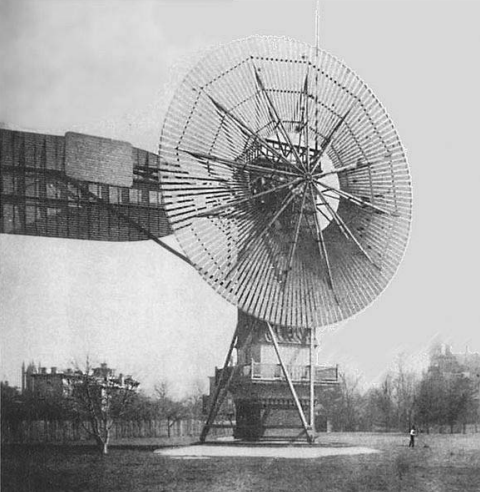
\includegraphics[height=8cm,width=10cm]{wt.png}
\caption{ توربین بادی 12 کیلو‌وات (ساخته‌شده به وسیله‌ی چارلز فرانسیس براش) \cite{b1}.}
\label{wt}
\centering
\end{figure}

یک نمونه از توربین‌های بادی اولیه در شکل~\ref{wt} نشان داده شده است. در \cite{a1}، یک مدل معیار\LTRfootnote{ Benchmark Model } برای پیاده‌سازی و مقایسه‌ی روش‌های تشخیص و جداسازی عیب در توربین‌های بادی ارائه شده است. این مدل معیار، یک توربین بادی سه پره‌ی  محور افقی با سرعت متغیر و توان مجاز 4/8 مگا‌وات را که به کنترل گام\LTRfootnote{ Pitch Control }(تغییر زاویه‌ی پره‌‌های توربین بادی حول محور طولی پره‌ها با اعمال فرامین کنترلی) نیز مجهز است، شبیه‌سازی می‌کند. هدف از ارائه‌ی این مدل، بوجود آوردن یک فضای مناسب برای مقایسه و آزمایش روش‌های مختلف تشخیص و جداسازی عیوب بر روی توربین است. از این مدل می‌توان برای مقایسه‌ی روش‌های سازش با عیب که در زمینه‌ی توربین بادی ارائه شده‌اند، استفاده کرد. تعداد زیادی از تحقیقاتی که در سال‌های گذشته در زمینه‌ی تشخیص و جداسازی عیب و همچنین سازش با عیب انجام گرفته است، طرح‌های پیشنهادی خود را بر روی این مدل آزمایش و مقایسه کرده‌اند. 

یکی از اجزای توربین بادی که در معرض عیب قرار دارد، محرک گام پره‌ی توربین می‌باشد. هر یک از پره‌های توربین بادی توسط یک محرک کنترل می‌شوند و با وقوع عیب در  محرک‌ گام هر پره، موقعیت گام آن پره با خطای زیادی مواجه می‌شود. برای حل این مساله،  در \cite{a10} یک روش جبران مبتنی بر تخصیص کنترل\LTRfootnote{ Control Allocation } ارائه شده است. تخصیص کنترل، یکی از رایج‌ترین روش‌های کنترل انعطاف‌پذیر در برابر عیب است. در روش پیشنهادی، گشتاوری که بر اثر عیب یکی از محرک‌ها اتلاف می‌شود، توسط اعمال قانون کنترلی به دو محرک دیگر جبران می‌گردد و توان مطلوب توربین بادی قابل دست‌یابی است.



\section{اهداف و دستاوردهای تحقیق}
از آنجایی که کنترل‌کننده‌ی توربین بادی برای تعیین ناحیه‌ی کنترلی و اعمال دستورات کنترلی مناسب، از اطلاعات حاصل از حس‌گر‌ها استفاده می‌کند؛ وقوع عیب در حس‌گر‌ها می‌تواند سبب تغذیه‌ی اشتباه کنترل‌کننده‌ی توربین شود. در صورتی که کنترل‌کننده‌ی توربین از اطلاعات اشتباه حس‌گر‌ها استفاده کند، دستورات کنترلی که به محرک‌ها اعمال می‌کند اشتباه خواهند بود. این امر سبب می‌شود تا با گذشت زمان، کل سیستم تحت تاثیر قرار گرفته و از حالت بدون عیب فاصله بگیرند. 

در این پایان‌نامه، طرحی پیشنهاد شده است که باعث جلوگیری از کاهش راندمان سیستم، در صورت وجود عیب در حس‌گر‌های اطراف پیشرانه‌ی توربین بادی خواهد شد. در این تحقیق، تشخیص زمان و مکان وقوع عیب، شدت عیب و جداسازی عیب‌ها از یکدیگر به صورت آنلاین مورد بررسی قرار گرفته است. با فرض این که حس‌گر‌های سرعت روتور و ژنراتور و همچنین گشتاور ژنراتور (حس‌گر‌های اطراف پیشرانه‌ی توربین بادی) دچار عیب شوند، با مدل‌سازی مناسب پیشرانه، رویتگر‌هایی را برای تخمین حالت و تولید مانده طراحی کرده و با کمک این رویتگر‌ها (که از نوع رویتگر‌های ورودی ناشناخته هستند)، برای هر یک از حس‌گر‌ها به طور جداگانه سیگنال آشکارسازی عیب تولید می‌کنیم. 

آشکارسازی آنلاین  و سازش با عیوب حس‌گر که در این پایان‌نامه ارائه شده است، بر روی مدل معیار توربین بادی پیاده‌سازی شده و با روش‌های دیگر مورد مقایسه قرار گرفته است. نتایج شبیه‌سازی، بهبود عملکرد سیستم را در صورت بکار‌گیری روش پیشنهادی نشان خواهد داد. 


\section{ساختار پایان‌نامه}
در فصل دوم  به طور مختصر با تاریخچه‌ی انرژی باد آشنا خواهیم شد. همچنین نحوه‌ی عملکرد توربین بادی و اجزای تشکیل‌دهنده‌ی توربین را نیز در این فصل بررسی خواهیم کرد. در پایان این فصل با انواع تقسیم‌بندی‌های توربین‌های بادی از نظر مکان نصب و نحوه‌ی اتصال به شبکه و قرار‌گیری روتور توربین به طور مختصر آشنا خواهیم شد.

در فصل پایانی به بیان نتایج پایان‌نامه و ارائه چند پیشنهاد پرداخته خواهد شد. 


% Chapter 2
\chapter{کنترل‌کننده بهینه $\mathcal{H}_2$}

یک سیستم زمان‌پیوسته در شکل~\ref{pic2-1} نشان داده شده است. این سیستم را به فرم استاندارد نیز می‌توان نمایش داد. در این فرم که در شکل~\ref{pic2-2} نشان داده شده است، سیگنال $w$ ورودی‌های خارجی سیستم نظیر ورودی مرجع\LTRfootnote{Reference Input}، نویز و اختلال را شامل می‌شود. $z$ سیگنالی است که قرار است کنترل شود و معمولاً خطای سیستم (اختلاف بین خروجی مطلوب و خروجی واقعی) است. $y$ ورودی کنترل‌کننده و $u$ نیز سیگنالی است که کنترل‌کننده آن را تولید می‌کند و به سیگنال کنترل معروف است. هم‌چنین در این فرم به دلیل این‌که سیستم $G$ دو ورودی و دو خروجی دارد، می‌توان آن را به چهار بخش به صورت 
\begin{equation*}
G=
\begin{bmatrix}
G_{11}&G_{12}\\G_{21}&G_{22}
\end{bmatrix} 
\end{equation*}
تقسیم کرد. در این صورت روابط
\begin{equation*}
\left\{\begin{array}{l}
z=G_{11}w+G_{12}u\\
y=G_{21}w+G_{22}u
\end{array}\right. 
\end{equation*}
بین ورودی‌ها و خروجی‌ها برقرار است.

\setlength{\unitlength}{1cm}
\begin{figure}[t]
\centering
\lr{
\begin{picture}(10.5,2.3)(0,0)
\put(0,1.5){\vector(1,0){1.35}}
\put(0.675,1.7){\makebox(0,0)[b]{$r(t)$}}
\put(1.2,1.7){\makebox(0,0){$ \scriptstyle + $}}
\put(1.5,1.5){\circle{0.3}}
\put(1.65,1.5){\vector(1,0){1.35}}
\put(2.325,1.7){\makebox(0,0)[b]{$e(t)$}}
\put(3,1){\framebox(1.5,1){$K(t) $}}
\put(4.5,1.5){\vector(1,0){1.5}}
\put(5.25,1.7){\makebox(0,0)[b]{$u(t)$ }}
\put(6,1){\framebox(1.5,1){$G(s)$}}
\put(7.5,1.5){\line(1,0){1.5}}
\put(9,1.5){\circle*{0.08}}
\put(9,1.5){\vector(1,0){1.5}}
\put(9.75,1.7){\makebox(0,0)[b]{$y(t)$}}
\put(9,1.5){\line(0,-1){1.5}}
\put(9,0){\line(-1,0){7.5}}
\put(1.5,0){\vector(0,1){1.35}}
\put(1.3,1.2){\makebox(0,0){$ \scriptstyle - $}}
\end{picture}
}
\caption{یک سیستم زمان‌پیوسته}
\label{pic2-1}
\end{figure} 

\setlength{\unitlength}{1cm}
\begin{figure}[b]
\centering
\lr{
\begin{picture}(5.4,4)(0,0)
\put(2,2.2){\framebox(1.4,1.4){$G$}}
\put(0,3.3){\vector(1,0){2}}
\put(1,3.5){\makebox(0,0)[b]{$w$}}
\put(3.4,3.3){\vector(1,0){2}}
\put(4.4,3.5){\makebox(0,0)[b]{$z$}}
\put(3.4,2.5){\line(1,0){1.5}}
\put(4.9,2.5){\line(0,-1){2}}
\put(5.1,1.5){\makebox(0,0)[l]{$y$}}
\put(4.9,0.5){\vector(-1,0){1.7}}
\put(2.2,0){\framebox(1,1){$K$}}
\put(2.2,0.5){\line(-1,0){1.7}}
\put(0.5,0.5){\line(0,1){2}}
\put(0.3,1.5){\makebox(0,0)[r]{$u$}}
\put(0.5,2.5){\vector(1,0){1.5}}
\end{picture}
}
\caption{یک سیستم زمان‌پیوسته در فرم استاندارد}
\label{pic2-2}
\end{figure} 


کنترل‌کننده بهینه $\mathcal{H}_2$، یک کنترل‌کننده علی و مناسب\LTRfootnote{Proper} است که سیستم را به‌طور داخلی پایدار کند و هم‌چنین به‌وسیله آن نرم $\mathcal{H}_2$ تابع تبدیل از  $z$ به $w$ ($T_{zw}$) مینیمم شود. به‌طور معادل می‌توان گفت کنترل‌کننده‌ای است که نرم دو پاسخ ضربه سیگنال  $z$ را مینیمم کند~\cite{paper_4}. در صورتی که سیستم متغیر با زمان باشد، تابع تبدیل مفهومی ندارد و از پاسخ ضربه باید استفاده کرد.  

%%%%%%%%%%%%%%%%%%%%%%%%%%%%%%%
%%%%%%%%%%%%%%%%%%%%%%%%%%%%%%%
\section{کنترل‌کننده بهینه $\mathcal{H}_2$ برای سیستم‌های زمان‌پیوسته}
در این قسمت روش طراحی کنترل‌کننده بهینه $\mathcal{H}_2$ برای یک سیستم زمان‌پیوسته بیان می‌شود. بدین منظور ابتدا به تعریف نرم $\mathcal{H}_2$ برای سیستم‌های زمان‌پیوسته می‌پردازیم و پس از آن روش طراحی کنترل‌کننده را بیان می‌کنیم.
%%%%%%%%%%%%%%%%%%%%%%%%%%%%%%%%%%%%5
\subsection{تعریف نرم $\mathcal{H}_2$ برای سیستم‌های زمان‌پیوسته} 
برای یک سیستم خطی، تغییرناپذیر با زمان و پایدار $G$ که زمان‌پیوسته و تک ورودی-تک خروجی است، نرم $\mathcal{H}_2$ به صورت 
\newcommand{\norm}[1]{\lVert#1\lVert}
\begin{equation}
\norm{\hat{g}(s)}_{2}=\sqrt{\dfrac{1}{2\pi}\int_{-\infty}^{\infty}{{\vert \hat{g}(j\omega)\vert}^2}d\omega} 
\label{eq2-1}
\end{equation}
تعریف می‌شود. در این رابطه $\hat{g}(j\omega) $ پاسخ فرکانسی سیستم است. بر اساس خاصیت پارسوال\LTRfootnote{Parseval}،  نرم $\mathcal{H}_2$ یک سیستم پایدار، با نرم دو پاسخ ضربه آن برابر است. 
اگر 
$\hat{g}(s)$
تابع تبدیل یک سیستم زمان‌پیوسته پایدار و
$G\delta(t)$
پاسخ ضربه آن باشد، آن‌گاه رابطه
\begin{equation}
\norm{\hat{g}(s)}_{2}=\norm{G\delta(t)}_{2} = \sqrt{\int_{0}^{\infty}{{\vert G\delta(t)\vert}^2}d t} 
\label{eq2-2}
\end{equation}
برقرار است.

برای سیستم‌های چند ورودی-چند خروجی روابط کمی پیچیده‌تر می‌شوند. فرض کنید سیستم $G$، $m$ ورودی و $p$ خروجی داشته باشد. در این صورت ماتریس انتقال آن، $p$ سطر و $m$ ستون دارد. نرم $\mathcal{H}_2$ برای چنین سیستمی به صورت
\begin{equation*}
\norm{\hat{g}(s)}_{2}=\sqrt{\dfrac{1}{2\pi}\int_{-\infty}^{\infty}{trace\left[ \hat{g}^{*}(j\omega)\hat{g}(j\omega)\right] }d\theta} 
\end{equation*}
تعریف می‌شود. در این رابطه، $\hat{g}(s)$ ماتریس انتقال سیستم است. هم‌چنین طبق خاصیت پارسوال اگر سیستم پایدار باشد رابطه 
\begin{equation}
\norm{\hat{g}(s)}_{2}=\sum_{i=1}^{m}{\norm{G\delta(t)e_{i}}_{2}} 
\label{eq2-3}
\end{equation}
نیز برای آن برقرار است. در این رابطه $e_{i}$ها بردارهای پایه استاندارد در فضای $\mathbb{R}^{m}$ هستند. $\delta(t)e_{i}$ تابع ضربه‌ای است که به ورودی $i$ام اعمال شده و $G\delta(t)e_{i}$ خروجی مربوط به آن است.

در صورتی که سیستم پایدار باشد، می‌توان از فضای حالت سیستم نیز برای محاسبه نرم $\mathcal{H}_2$ استفاده کرد.  فرض کنید معادلات فضای حالت یک سیستم پایدار به صورت 
\begin{equation*}
\left\{\begin{array}{l}
\dot{x}=Ax +Bu\\
y =Cx+Du 
\end{array}\right. 
\end{equation*}
باشد که $x$ بردار حالت سیستم، $u$ بردار ورودی و $y$ بردار خروجی است. $A$ نیز یک ماتریس هرویتز\LTRfootnote{Hurwitz} است. هم‌چنین برای محدود بودن نرم $\mathcal{H}_2$ سیستم زمان‌پیوسته، $D$ باید صفر باشد. در این صورت برای محاسبه نرم $\mathcal{H}_2$ سیستم، می‌توان از روش زیر استفاده کرد \cite{book_1}: 
\begin{enumerate}
\item
حل معادله لیاپانوف زمان‌پیوسته\LTRfootnote{Continuous-time Lyapunov Equation} ($AL+LA^{T}+BB^{T}=0$) و یافتن ماتریس نامعلوم $L$.
\newline
باید دقت شود که در صورت هرویتز بودن ماتریس $A$، معادله لیاپانوف حل یکتا دارد.
\item
محاسبه نرم  $\mathcal{H}_2$از طریق رابطه $\norm{\hat{g}}_{2}=\sqrt{trace(CLC^{T})}$.
\end{enumerate}
%%%%%%%%%%%%%%%%%%%%%%%%%%%%%


% Appendices
\appendix
% Appendix 1
\chapter{تبدیل دوخطی}

یکی از روش‌های گسسته‌سازی یک سیستم زمان‌پیوسته روش تبدیل دوخطی است. این روش که به روش توستین\LTRfootnote{Tustin} نیز معروف است، یک روش انتگرال‌گیری عددی به کمک تقریب ذوزنقه‌ای است. سیستمی با ورودی $u(t)$، خروجی $y(t)$ و تابع تبدیل $\dfrac{1}{s}$ در نظر بگیرید. رابطه
\begin{equation}
y(t)=\int_{-\infty}^{t}{u(\tau)} d \tau 
\label{eq2-19}
\end{equation}
بین ورودی و خروجی سیستم برقرار است. با گسسته‌سازی \ref{eq2-19} به رابطه
\begin{equation}
y[(k+1)h]=y(kh)+\int_{kh}^{(k+1)h}{u(\tau)} d \tau 
\label{eq2-20}
\end{equation}
می‌رسیم. اگر از تقریب ذوزنقه‌ای برای محاسبه انتگرال استفاده کنیم، \ref{eq2-20} به صورت 
\begin{equation}
y[(k+1)h] \simeq y(kh)+\dfrac{h}{2}\left(u(kh)+u[(k+1)h]\right)
\label{eq2-21}
\end{equation}
در می‌آید. از رابطه تقریبی \ref{eq2-21} می‌توان برای تبدیل یک سیستم زمان‌پیوسته به یک سیستم زمان‌گسسته استفاده کرد.

سیستم زمان‌پیوسته خطی و تغییرناپذیر با زمان $G=(A,B,C,D)$  را در نظر بگیرید. اگر این سیستم را با دوره تناوب $h$ گسسته‌سازی کنیم، مدل فضای حالت $G_d=(A_d,B_d,C_d,D_d)$ به دست می‌آید که در آن
\begin{equation*}
A_{d}=(I-\dfrac{h}{2}A)^{-1}(I+\dfrac{h}{2}A) 
\end{equation*} 
 \begin{equation*}
B_{d}=\dfrac{h}{2}(I-\dfrac{h}{2}A)^{-1}B) 
\end{equation*} 
  \begin{equation*}
C_{d}=C(I+A_{d}) 
\end{equation*} 
  \begin{equation*}
D_{d}=D+CB_{d} 
\end{equation*} 
 است.


% References
\renewcommand{\bibname}{مراجع}
\addcontentsline{toc}{section}{مراجع}

\begin{thebibliography}{99}

\begin{latin}

\baselineskip=.7cm

\bibitem{b6}
\noindent Isermann, R., \textit{Fault Diagnosis Systems An Introduction from Fault Detection to Fault Tolerance}, Springer, Berlin, 2006.

\bibitem{b1}
Shea, K., and Howard, B.C., \textit{Build Your Own Small Wind Power System}, McGraw-Hill Professional, 2011.

\bibitem{a1} 
Odgaard, P. F., Stoustrup, J., and Kinnaert, M., “Fault-tolerant control of wind turbines: A benchmark model”,  \textit{IEEE Transactions on Control Systems Technology}, Vol.~21, No.~4, pp.~1168–1182, 2013.

\bibitem{a10}
Jiyeon, K., and Yang, I., “Control allocation based compensation for faulty blade actuator of wind turbine”, in \textit{8th IFAC Symposium on Fault Detection, Supervision and Safety of Technical Processes}, pp.~355–360, 2012.

\bibitem{book_1}
Zhou, K., and Doyle, J.C., \textit{Essentials of Robust Control}, Prentice-Hall, 1998.


\bibitem{paper_4}
Hespanha, J.P., Naghshtabrizi, P., and Xu, Y., ``A survey of recent results in networked control systems", \textit{IEEE Proceedings}, Vol.~95, No.~1, pp.~138-162, 2007.

\end{latin}


\bibitem{ref3}
عالمی، ح، "اثر اغتشاش در سیستم‌های مخابراتی``، \textit{استقلال،} دانشگاه صنعتی اصفهان، شماره~5، صص~27-34، 1361.

\end{thebibliography}

\addcontentsline{toc}{section}{چکیده انگلیسی}
\thispagestyle{empty}

\begin{latin}
\begin{center}

{\Huge Increasing Efficiency in Low-Efficiency Systems}

\vspace{1cm}

{\LARGE{Azin Azadeh}}

\vspace{0.2cm}

{\small azin.azadeh@ec.iut.ac.ir}

\vspace{0.5cm}

March 21, 2015

\vspace{0.5cm}

Department of Electrical and Computer Engineering

\vspace{0.2cm}

Isfahan University of Technology, Isfahan 84156-83111, Iran

\vspace{0.2cm}

Degree: M.Sc. \hspace*{3cm} Language: Farsi

\vspace{1cm}

{\small\textbf{Supervisor: Prof. Bahram Borzou (bahram.borzou@cc.iut.ac.ir)}}
\end{center}
~\vfill



\noindent\textbf{Abstract}

\begin{small}
\baselineskip=0.6cm
In most applications, because of numerous advantages it offers,
digital technology (computer, PLC, microcontroller etc.) is used to
control industrial plants. These types of systems, where the process
under control is continuous-time but the controller is digitally
implemented, are called sampled-data systems. Faults can occur in
sampled-data systems like any other control system. In order to
prevent performance degradation, physical damage or failure, faults
should be promptly detected. In this thesis fault diagnosis in
sampled-data systems is studied. The sampled-data design can be
carried out using direct or indirect design approaches. Direct
design, emphasized in this research, does not involve any
approximations.

Normally, to design a robust fault detection and isolation (FDI)
scheme, a performance index which is a measure of the sensitivity of
the FDI to faults and its robustness to unknown inputs and
disturbances is defined and optimized. Different performance indices
based on norms are considered. Using the direct design
approach and the so-called norm invariant transformation, it is
shown that a sampled-data FDI problem can be converted to an
equivalent discrete-time problem. This will form the foundation of a
unifying framework for optimal sampled-data residual generator
design.

Multirate systems are also abundant in industry. Here, several
methods of residual generation based on multirate sampled data are
developed. The key feature of such residual generators is that they
operate at a fast rate for prompt fault detection. The lifting
technique is used to convert the multirate problem into an
equivalent single-rate discrete-time problem with causality
constraints.

It is generally believed that the optimal multirate design performs
better than the optimal slow-rate and worse than the optimal
fast-rate designs. This conjecture is theoretically proved in this
thesis for general multirate control systems with norms of the
closed-loop system as performance indices. However, it is shown that
the common performance indices in FDI design do not satisfy this
property. To resolve this, an alternative performance index is
defined after formulating the FDI problem as a standard control
problem.

\end{small}

\vspace{0.5 cm}

\noindent \textbf{Key Words}: Fault Detection, Wind Turbine Control, Fault Accomodation, Unknown Input Observers

\end{latin}

%********************************
% Page before last: English Signatures
%********************************
\thispagestyle{empty}
\newgeometry{left=3cm,right=3cm,top=2cm}
\begin{latin}
\begin{center}

\includegraphics[height=3cm]{iut_logo.png}
\vspace{0.4cm}

{\large\textbf{Isfahan University of Technology}}\\

\vspace{0.4cm}
Department of Electrical and Computer Engineering

\vspace{2.5cm}

{\Huge Increasing Efficiency in Low-Efficiency Systems}

\vspace{1.5cm}

{\large
	A Thesis
	
	\vspace{.3cm}
	
	Submitted in partial fulfillment of the requirements
	
	\vspace{.3cm}
	
	for the degree of Master of Science
}

	\vspace{1.5cm}

{\Large
	\textbf{by}
	
	\vspace{.3cm}
	
	\textbf{Azin Azadeh}
}
\end{center}

\vfill

Evaluated and Approved by the Thesis Committee, on March 21, 2015
\vspace{0.5cm}

\begin{enumerate}
\item Bahram Borzou, Prof. (Supervisor)
\vspace{0.5cm}

\item Poorya Parniani, Assoc. Prof. (Advisor)
\vspace{0.5cm}

\item Tahamtan Trabi, Prof. (Examiner)
\vspace{0.5cm}

\item Soraya Sanaei, Assist. Prof (Examiner)
\vspace{0.5cm}

\end{enumerate}

Jamshid Jahangir, Department Graduate Coordinator

\pagebreak
\end{latin}

%***************************
% last page: Blank
%***************************
\thispagestyle{empty}
\mbox{}

% It's finally over. Wasn't that hard, was it?

\end{document}